\begingroup
\setbeamertemplate{headline}{%
	\leavevmode%
	\hbox{%
		\begin{beamercolorbox}[wd=\paperwidth,ht=2.5ex,dp=1.25ex]{palette tertiary}%
			\centering
			\hyperlink{extras}{Backup Sheets}
		\end{beamercolorbox}%
	}
}

\appendix

\begin{frame}
\hypertarget{extras}{}
	\frametitle{Bayesian Optimization}
	\begin{itemize}
		\item Given an expensive, unknown objective function $f: \mathcal{X} \mapsto \mathbb{R}$ ($\mathcal{X} \subset \mathbb{R}^m$)
		\item Find global maximizer $x^* \in \mathcal{X}$ s.t.:
		\begin{align*}
		x^* &= \arg\max_{x \in \mathcal{X}} f(x)
		\end{align*}
		\item Bayesian Optimization components:
		\begin{itemize}
			\item \textit{Prior over $f$}: Gaussian Process $f \sim GP(\mu(\cdot), K(\cdot, \cdot))$	% (Gaussian) probability distribution over functions
			\item \textit{Evidence set}: $\mathcal{D}_{1:t} = \{(x_i, y_i) \mid i = 1 \ldots t\}$
			\item \textit{Posterior} or \textit{Surrogate function} ('estimate of $f$')
			\item \textit{Acquisition} or \textit{Utility function}: $u: \mathcal{X} \mapsto \mathbb{R}$ 
		\end{itemize}
	\end{itemize}
\end{frame}

\begin{frame}{Bayesian Optimization}{Toy Example}
\vspace{-8pt}
\begin{center}
	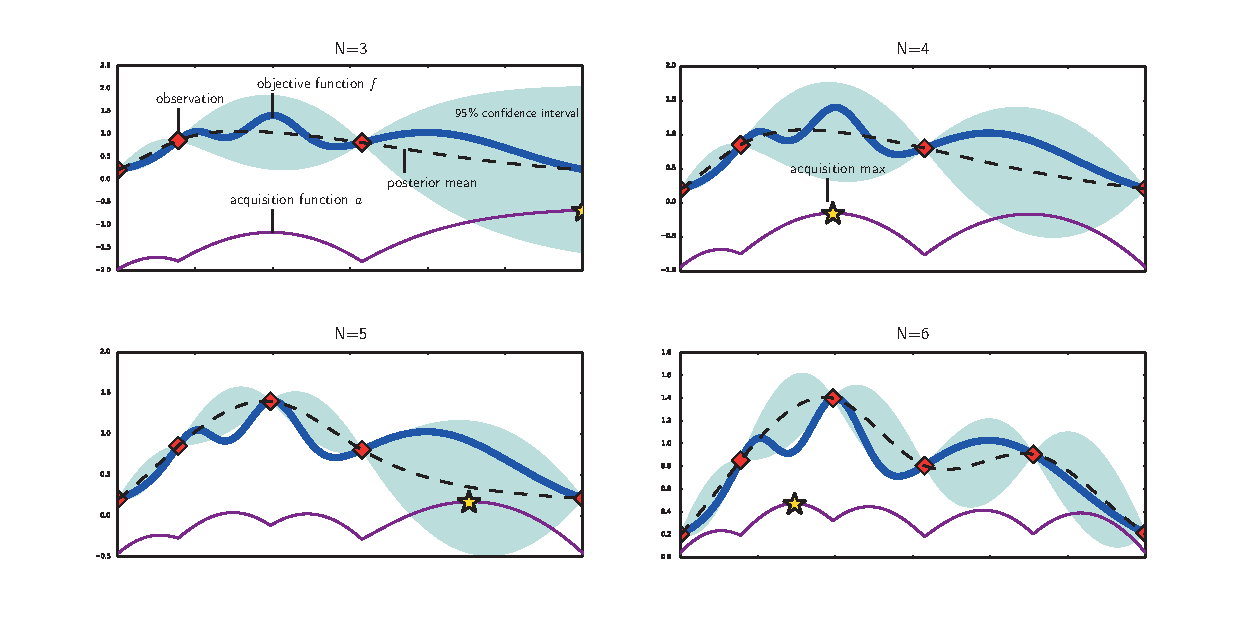
\includegraphics[width=\textwidth]{figures/bo_toy_example_v1.pdf}
\end{center}
\end{frame}

\begin{frame}{Bayesian Optimization}{Acquisition Functions}

Let $f(x^+)$ be the best observation, then the acquisition functions sample the maximizer $x$ of the following quantities:

\begin{labeling}{\textbf{Expected Improvement Per Second (EIPS)}}
	\item[\textbf{Probability of Improvement (PI)}] $P(f(x) \geq f(x^+) + \xi)$
	\item[\textbf{Expected Improvement (EI)}] $\mathbb{E}[\max(0, \mu_f(x) - f(x^+) - \xi)]$
	\item[\textbf{GP Upper Confidence Bound (GP-UCB)}] $\mu_f(x) + \beta\sigma_f(x)$
	\item[\textbf{Expected Improvement Per Second (EIPS)}] $\textsc{EI}(x) / \mu_s(x)$
\end{labeling}

where $\xi \geq 0$ is an exploration-exploitation trade-off parameter, $\beta \geq 0$ specifies number of standard deviations, $\mu_s$ is the mean of a timing GP.
	
\end{frame}

\begin{frame}{Automated Model Checking}{Objective}
\textbf{Goal:} Compose algorithms that construct probabilistic models which (partially) satisfy temporal goals.

\begin{itemize}
	\item Temporal goals expressed through LTL formulas
	\item Example: $\varphi = (a \mathbin{\mathcal{U}\kern-.1em} b) \wedge \mathbin{\mathcal{X}\kern-.1em} c$ \\ ``$a$ should hold until $b$ is true after which $c$ should become true''
\end{itemize}
%\begin{columns}
%	\begin{column}{0.5\textwidth}
%		content...
%	\end{column}
%\end{columns}
\end{frame}

\begin{frame}{Automated Model Checking}{Example Lacerda et al. \cite{lacerda2015optimal}}
	\begin{center}
		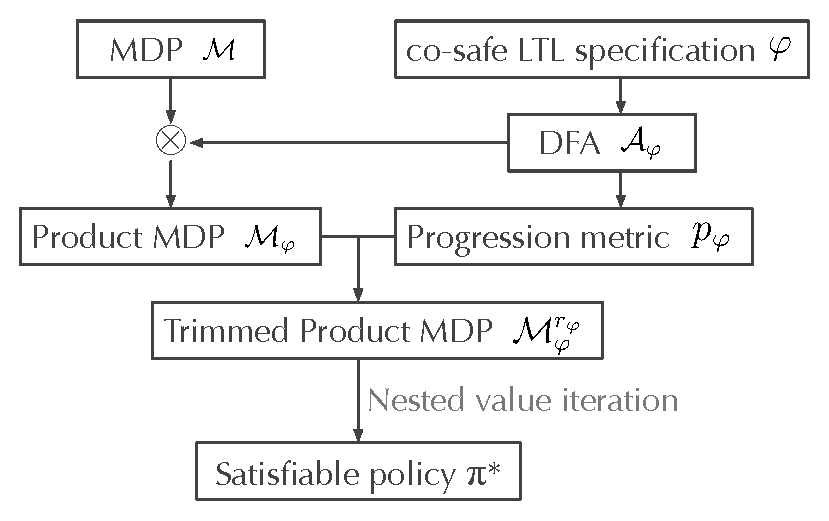
\includegraphics[width=0.6\textwidth]{figures/productMDP.eps}
	\end{center}
\end{frame}

\begin{frame}
\frametitle{Model Optimization Framework}
\framesubtitle{MDP Finetuning Example}

\begin{columns}
	\begin{column}{0.5\textwidth}
		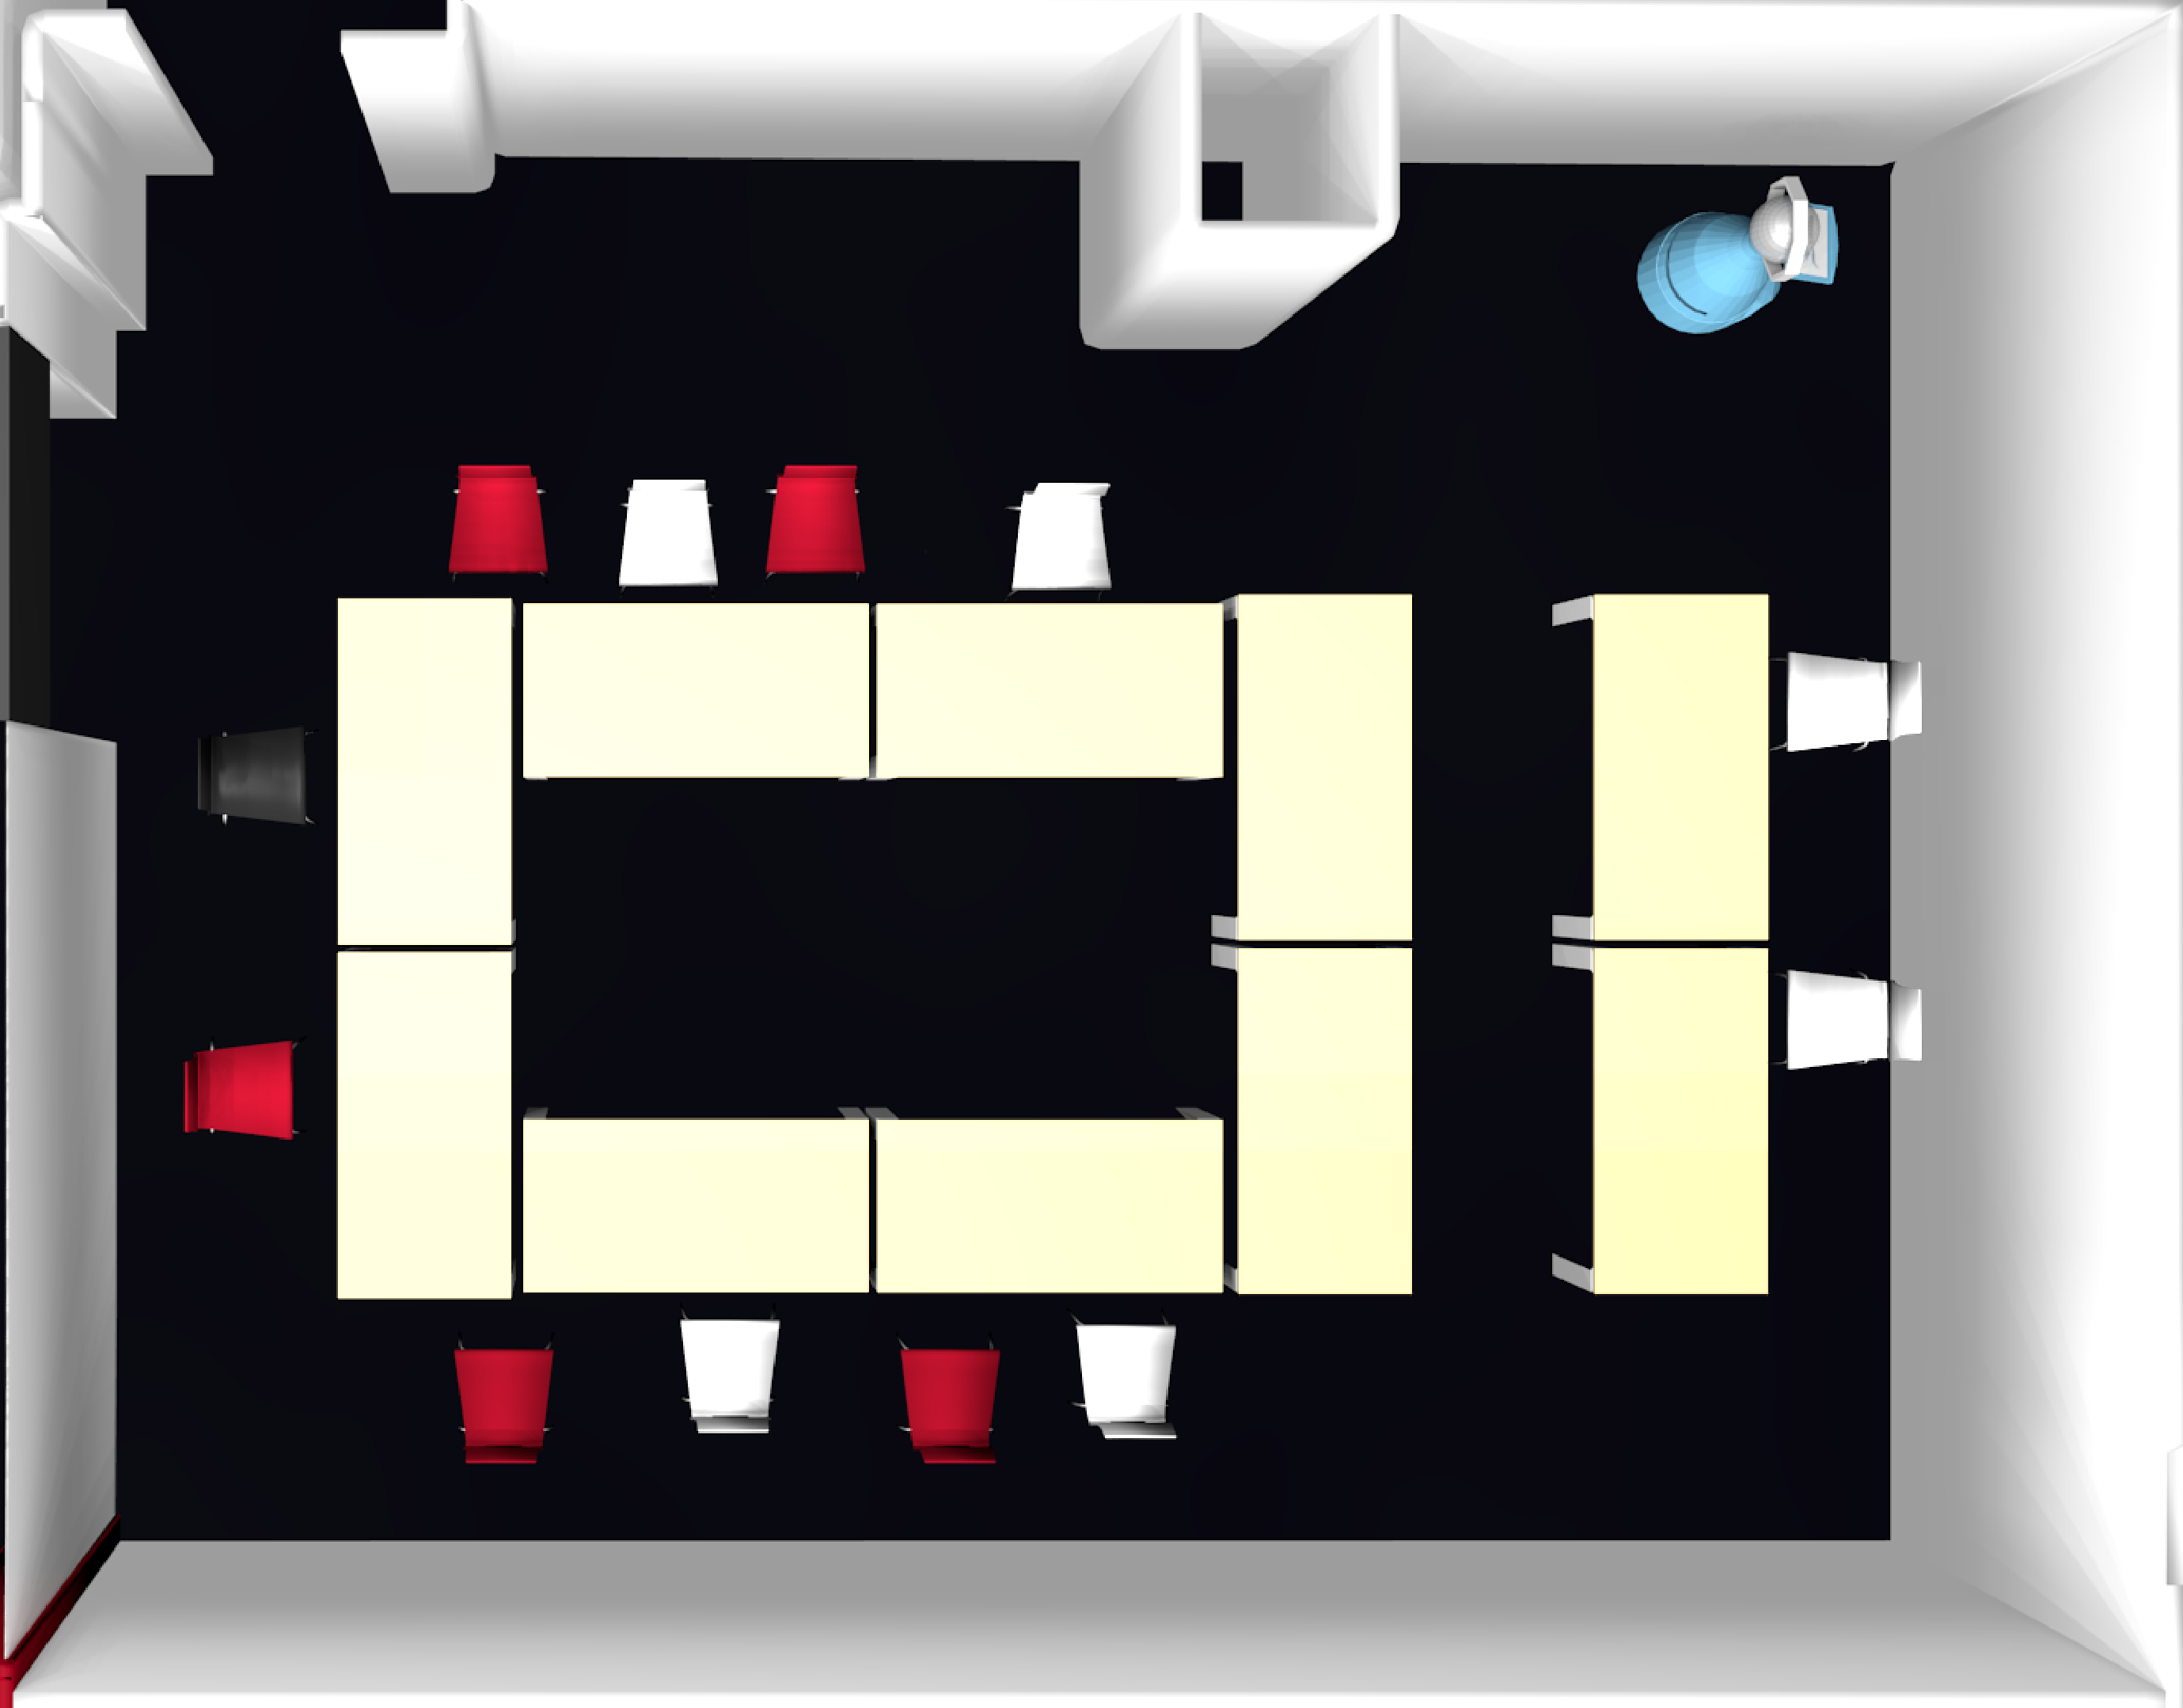
\includegraphics[width=0.95\textwidth]{figures/implementation/uol_bl_phase_3_small}
	\end{column}
	\begin{column}{0.5\textwidth}
		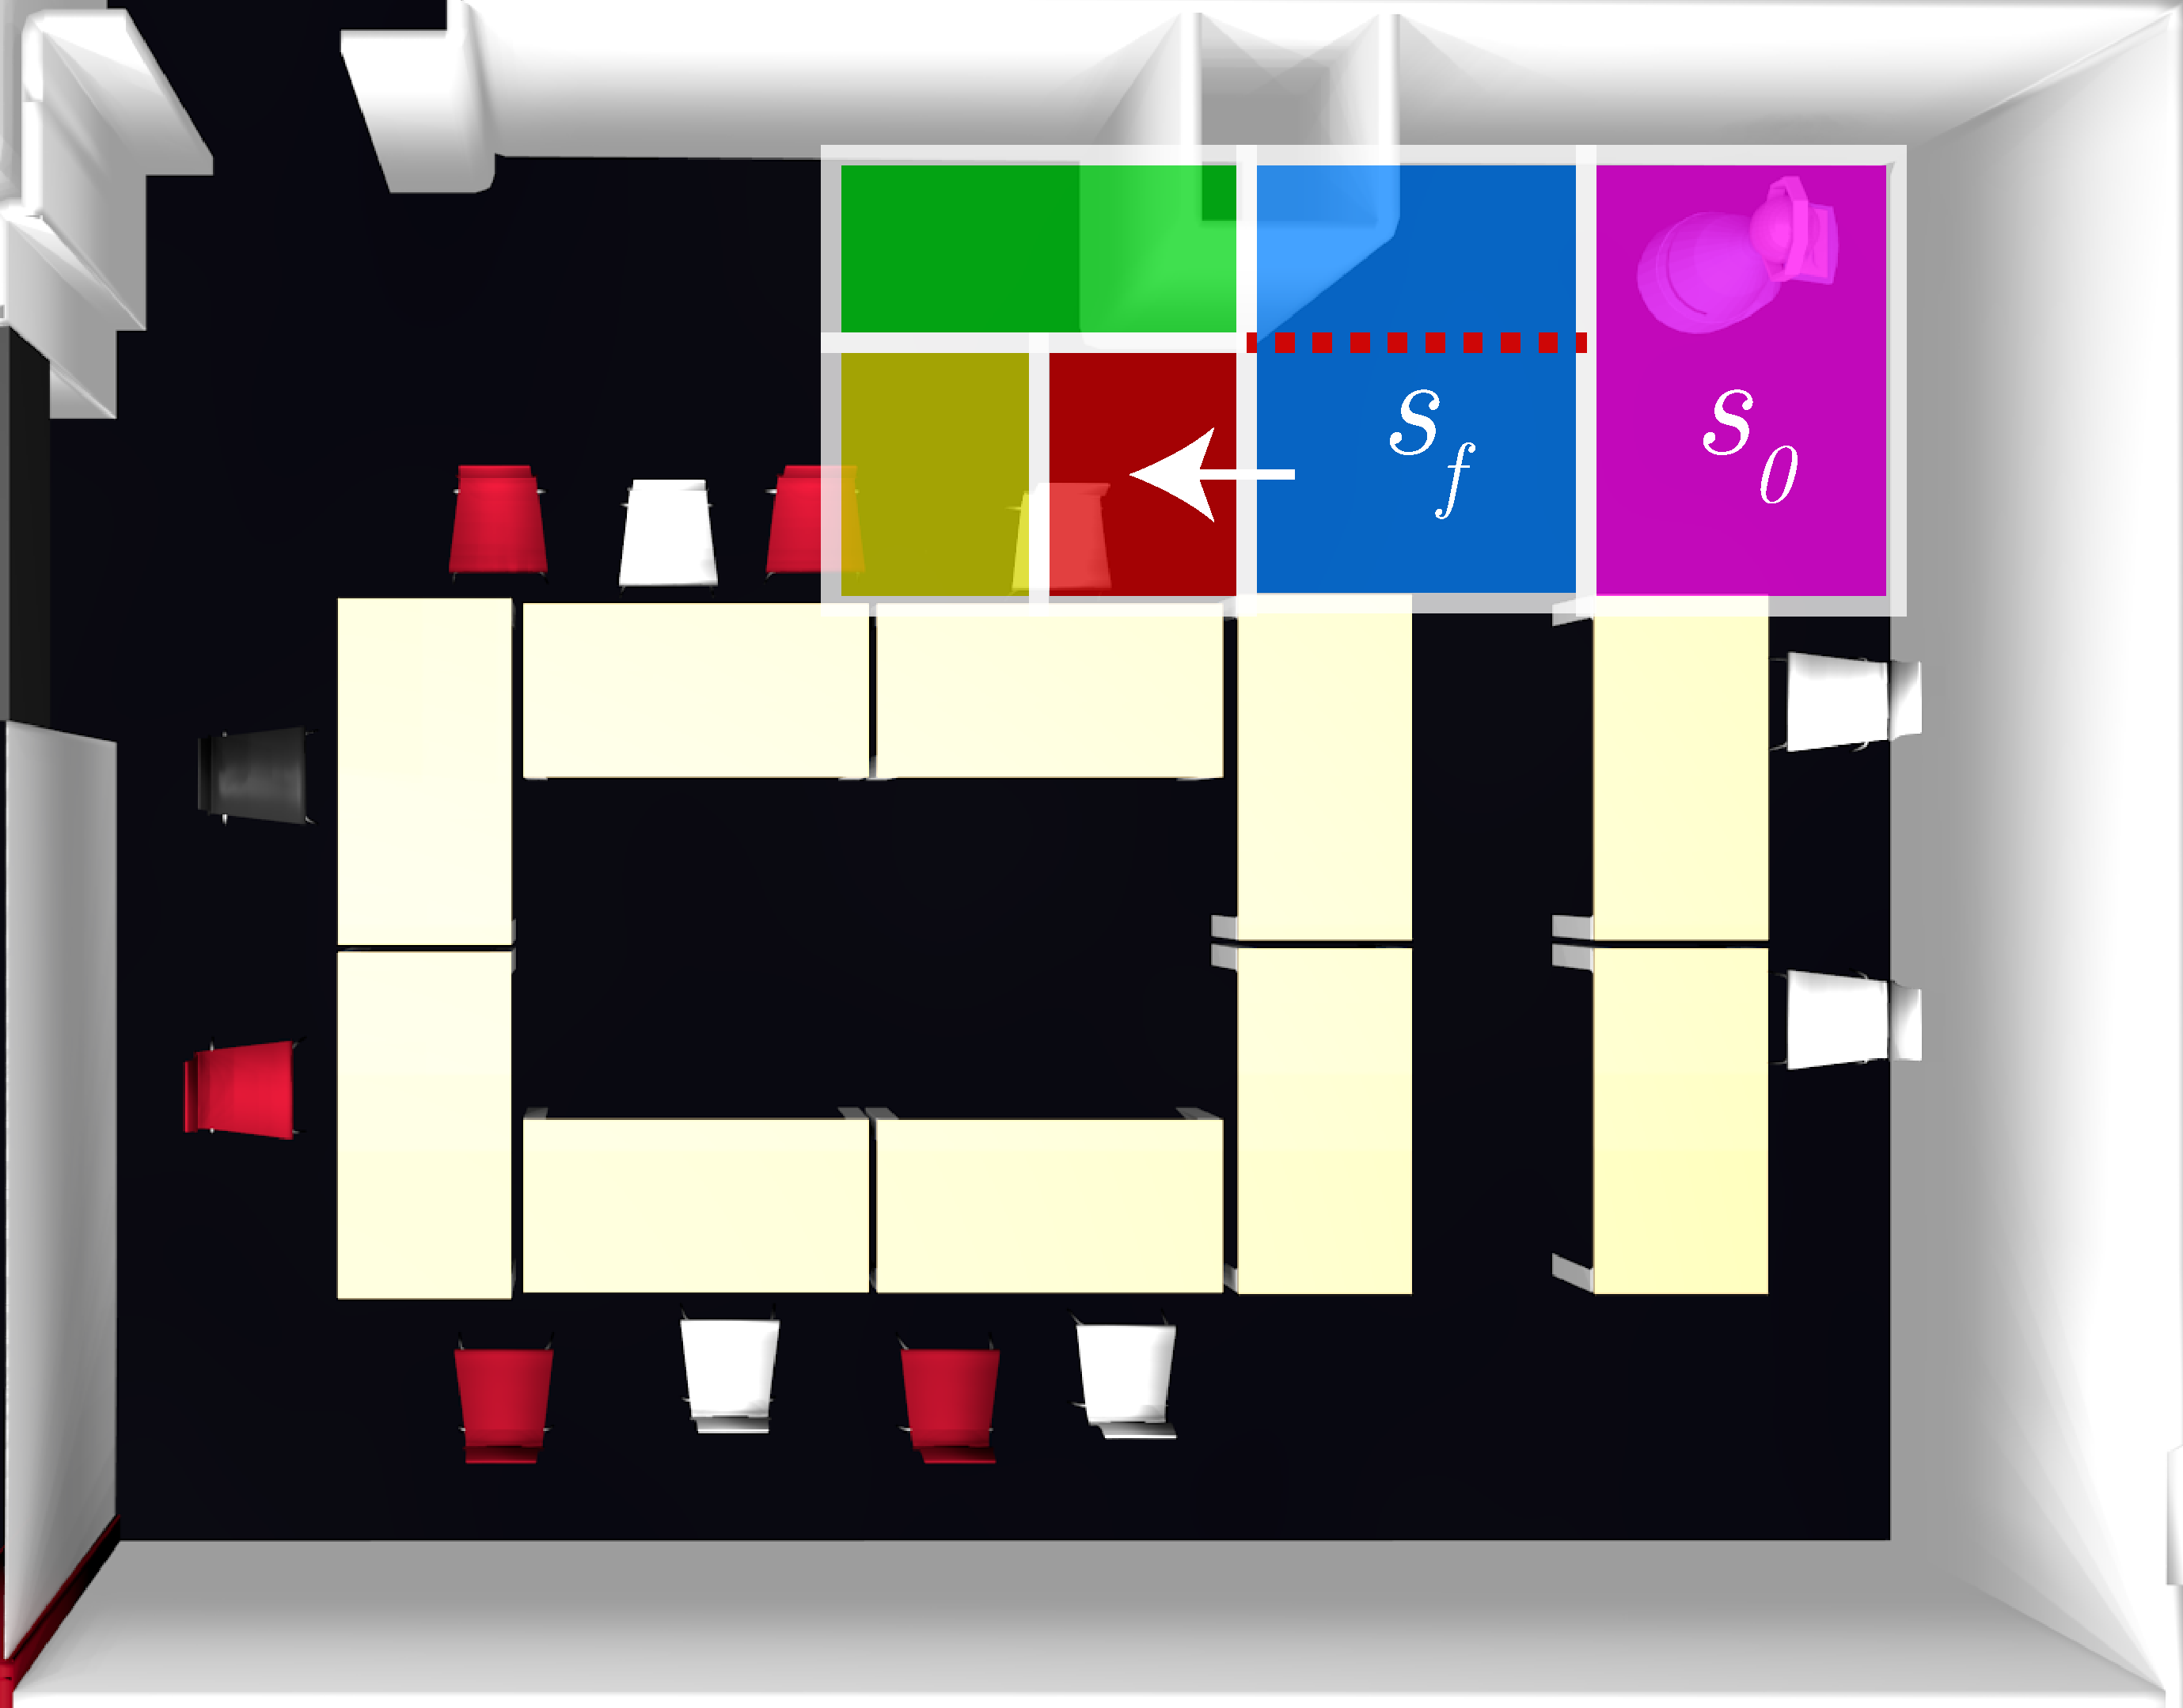
\includegraphics[width=0.95\textwidth]{figures/implementation/uol_bl_phase_3_2_smallv6.pdf}
	\end{column}
\end{columns}

\end{frame}

\begin{frame}{Model Learning Algorithms}{Baum-Welch for HMMs/POMDPs}
	\textbf{Goal}: Maximize $P(\lambda \vert O)$ with $\lambda$ the model parameters and $O$ the observation sequences
	\vspace{10pt}
	
	High-level steps:
	\begin{enumerate}
		\item Provide initial probability estimates
		\item Repeat the following until convergence:
		\begin{enumerate}
			\item \textit{E-step}: Compute expectations of how often transitions and emissions are used
			\item \textit{M-step}: Update parameters based on these expectations
		\end{enumerate}
	\end{enumerate}
\end{frame}

\begin{frame}{Model Learning Algorithms}{Baum-Welch for HMMs/POMDPs}
	\textbf{Goal}: Maximize $P(\lambda \vert O)$ with $\lambda$ the model parameters and $O$ the observation sequences
	\vspace{10pt}
	
	Detailed Steps \cite{welch2003hidden}:
	\begin{itemize}
		\item Compute the following quantities using the \textit{forward} and \textit{backward} procedures given observation sequences $O$ of length $T$:
		\begin{center}
			\begin{multicols}{2}
				$\xi_{ij}(t) = P(q_t = s_i, q_{t+1} = s_j)$
				\hspace{20pt}
				$\gamma_i(t) = \sum_{j=1}^{|\mathcal{S}|} \xi_{ij}(t)$
			\end{multicols}
		\end{center}
		

		\item Update model parameters as follows:
		\begin{center}
			\begin{multicols}{3}
				$a_{ij}(t) = \frac{\sum_{t=1}^{T-1} \xi_{ij}(t)}{\sum_{t=1}^{T-1} \gamma_{i}(t)}$
				\hspace{20pt}
				$b_{jk}(t) = \frac{\sum_{O_t = v_k} \gamma_j(t)}{\sum_{t=1}^{T} \gamma_j(t)}$
				\hspace{20pt}
				$\pi_i = \gamma_i(1)$
			\end{multicols}
		\end{center}
		
	\end{itemize}
\end{frame}

\begin{frame}{Model Learning Algorithms}{Time-State Merging / Model Merging}
\vspace{10pt}
\begin{center}
	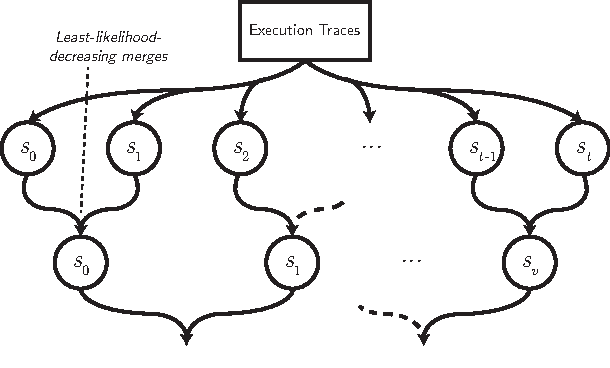
\includegraphics[width=0.65\textwidth]{figures/model-merging-bfmm}
\end{center}
\end{frame}

\begin{frame}{Factored MDPs}

\begin{columns}
	\begin{column}{0.5\textwidth}
\begin{definition}
	A Factored Markov Decision Process is a tuple $\mathcal{M} = (\mathcal{X}, s_0, A, T, R)$ in which:
	\begin{itemize}
		\item $\mathcal{X} = \{X_1, \ldots, X_n\}$ is a set of state variables (or \textit{features}) with $s_0 \in \mathcal{X}$
		\item $A$ is the action space
		\item $T: \mathcal{X} \times A \times \mathcal{X}$ is a transition function
		\item $R: \mathcal{X} \mapsto \mathbb{R}$ a reward function
	\end{itemize}
\end{definition}
\end{column}
\begin{column}{0.5\textwidth}
\begin{tikzpicture}[
node distance=1.5cm and 0cm,
state/.style={draw,ellipse,text width=1.8cm,align=center}
]
\node[state] (pos0) {$\textsc{Pos}[0]$};
\node[state,right=0cm and 1cm of pos0] (pos1) {$\textsc{Pos}[1]$};
\node[state, above of= pos0] (fire0) {$\textsc{Fire}[0]$};
\node[state, right=0cm and 1cm of fire0] (fire1) {$\textsc{Fire}[1]$};
\node[state, below of= pos0] (vis0) {$\textsc{Visitor}[0]$};
\node[state, right=0cm and 1cm of vis0] (vis1) {$\textsc{Visitor}[1]$};
\node[below of= vis0] (text0) {Decision epoch $t$};
\node[below of= vis1] (text1) {Decision epoch $t + 1$};
\path (pos0) edge[-latex] (pos1)
(pos0) edge[-latex] (vis1)
(pos0) edge[-latex] (fire1)
(fire0) edge[-latex] (fire1)
(vis0) edge[-latex] (vis1)
;
\end{tikzpicture}
\end{column}
\end{columns}

\end{frame}
\endgroup